\section{Linear Texture Mapping}

This section is divided into three parts, first we will look at how to overview the ITU logo on the image sequence of universities ground floor. Then we look at how we can overview a texture on a moving object. In the third part we tried to be sure that the texture looks realistic compared to the geometry of the texture.

\subsection{Ground Floor}

In this part we tried to overview the ITU logo on the image sequence of ground floor. For this we used the same code from simpleTextureMap function and declare the texturemapGroundFloor method with the implementation for overviewing the logo on each frame of the sequence by using four mouse input points from the first frame.

\begin{figure}[h!]
	\centering
	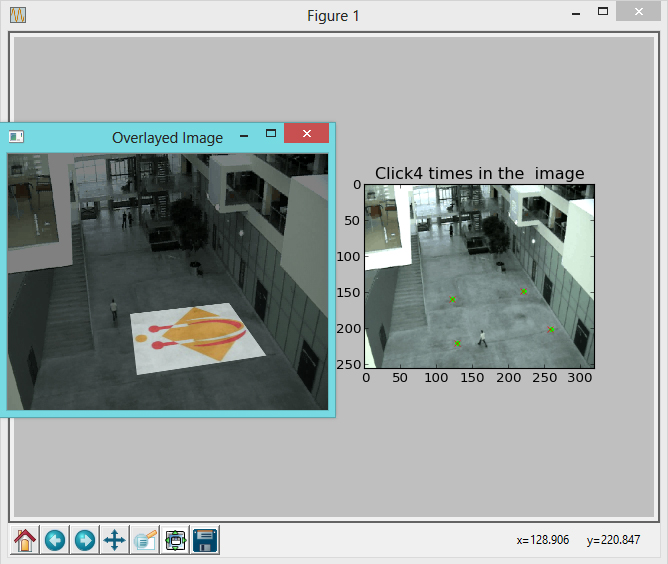
\includegraphics[width=\textwidth]{Handin2/images/linearmapping.jpg}
	\caption{Trace Map}
	\label{fig:trace}
\end{figure}

\subsection{Moving object}

In the second part of linear texture mapping we tried to experiment with texture mapping on image sequences where the objects move. We have been given some video files where a grid pattern moves in it. The aim is to mapping a texture on the pattern that will move with it. For the start we found the pattern corners with findChessboardCorners function and used it for calculating the homography matrix and overview the logo on the pattern. So for each frame we get a new homography matrix and new texture mapping.

\begin{figure}[h!]
	\centering
	\includegraphics[width=\textwidth]{Handin2/images/linearmapping-part2.jpg}
	\caption{Moving Pattern}
	\label{fig:trace}
\end{figure}

\subsection{Ensuring a correctly placed texturemap}
